\documentclass[aps,preprint,amsmath,amssymb]{revtex4}
%\documentclass[aps,twocolumn,amsmath,amssymb]{revtex4}
\usepackage{graphics}
\usepackage[pdftex]{graphicx}% Include figure files
\usepackage{bm}
\usepackage{natbib} % necessary for bibtex
\usepackage[toc,page]{appendix}

\begin{document}

\title{Visual Geolocation Based Black and White Listing}

\author{Karl Cronburg}
\email{karl@cs.tufts.edu}
\affiliation{Dept. of Computer Science, Tufts University, Medford MA 02155}

\begin{abstract}
Various commercial and open-source tools are available for managing IP-based
filtering of web traffic. A common open-source method is the 
use of static `tricks' found on stackoverflow (e.g. defining Apache rewrite
rules). A more involved approach is to create \emph{iptables} rules.
However, the availability of tools to interact with iptables from a
high level is lacking.
As such, we present a novel approach to managing iptables filtering
through an interactive map of the world powered by Google Maps
and IP2Location.com. Our approach focuses on effectively conveying
web site traffic in a way that any content-provider can understand, regardless of
prior experience with tools like iptables.
We discuss the effectiveness of existing black and whitelisting tools,
and where our approach fits into today's network security landscape.
We conclude with a discussion of possible improvements
to our approach, which should lead to increased productivity of website
administrators in dealing with network attacks. 
\end{abstract}

\maketitle

\section{Introduction}
The most common application of defense-in-depth is through the application of firewalls,
in particular firewalls with rules either blacklisting or whitelisting traffic based
on IP and DNS information associated with packets coming in and out of a network. The
purpose of a blacklist is usually to predict the source of future network-based attacks,
mitigating attacks before they have the chance to unfold.~\cite{DBLP:journals}
The types of network attacks mitigated can range from Denial of Service (asymmetric attacks)
to Cross-Site Scripting (application-specific attacks) and beyond.

Since blacklisting is predictive in nature, most research in this area is on pattern
matching and the compiling of databases of suspected attack patterns. As a result
blacklisting is susceptible to never before seen attacks coming from previously
unsuspected sources (which, when possible, is mitigated using whitelists). The techniques
for compiling and using databases of attack patterns are described by \cite{Zhang:2008}.
The primary techniques used today are known as GWOL and LWOL. \emph{GWOL} stands for
`Global Worst Offenders List', which focuses on institutions and users world-wide collaborating
in an effort to compile attack sources. Implementing GWOL is similar to implementing
a \emph{Web of Trust} for public key distribution; groups of institutions and users who
inherently trust each other exchange their network logs in an effort to paint the fullest
picture of the Internet. The second technique, \emph{LWOL}, stands for `Local Worst Offenders
List', which focuses on profiling attack patterns on a specific machine / subnet of the
Internet.

GWOL builds on the work of the already well-established LWOL technique, synthesizing
the information compiled by LWOL machines. The work of \cite{DBLP:journals} further builds
on the work of \cite{Zhang:2008} by looking for patterns \emph{across} network logs
rather than on an individual machine basis. The everlasting challenge with pattern
matching, however, is being able to put network traffic into context. While an
algorithm to match these patterns could take many years to perfect and subsequently
implement, a human can be trained to pick up on such patterns in a matter of days. 
A human can synthesize many different sources of both subjective and objective data
in a heartbeat whereas algorithms in IDSs today must be carefully fed every piece
of information they require and employ some complicated algorithm to compute objective
metrics. While long-term automation in this manner is certainly a noble pursuit, with
CS grad students and professors meticulously developing algorithms and publishing
groundbreaking papers over the years, the challenges of detecting and preventing attacks
\emph{today} remains an issue we need to solve either \emph{today} or in the
not-to-distant future.

This paper presents a proof-of-concept implementation of human-driven pattern matching /
blacklisting. The hope is that a complete implementation can be created in the course
of a couple months.

%Source~\cite{Zhang:2013}.
%Source~\cite{Peng:2008}.
%Source~\cite{Kim:2008}.

\section{To The Community}

%\subsection{HCI in Security}
%\begin{enumerate}
%\item HCI in Security
%\item User friendliness of security tools makes them more widely accessible
%\end{enumerate}

\subsection{Black \& White Listing Applications}

\begin{enumerate}
\item Most attempts to filter spam and block phishing incidents involve IP blacklists;
statistics about long-term trends in network traffic can be used to correlate IP addresses
into groups, specifically botnets.~\cite{West:2011} Using a visualization tool similar to
the one discussed in this paper is a possible way to look for patterns in the geographic
layout of a botnet, and to be able to compare the size, extent, and characteristics of
one botnet versus another.
\item Determining whether to use a whitelist or a blacklist is a key issue in various
situations. For instance in~\cite{Wu:2012} the efficienty of an academic document search engine
is determined when using a blacklist versus a whitelist. In this research, efficiency was
measured as the speed at which the crawler is able to index appropriate academic documents.
In this situation whitelisting was found to be more efficient with higher quality documents
indexed. In contrast, the blacklist had a low efficiency with many low quality documents, but
has a lower false-negative rate.
\item In~\cite{Zhang:2013} the impact of Real-time Blackhole Lists (RBLs) is discussed.
A RBL is simply a blacklist of IPs for which a subnet of the Internet will drop / ignore
all requests going to or from that IP address.
The discussion touches upon the affinity for certain RBLs to have very specific geographic
qualities / distributions. That is to say, RBLs for SPAM and certain active attacks tend
to contain a lot of Asian / Pacific and European IP addresses. In contrast phishing and
malware RBLs tend to contain a lot of North American IP addresses.~\cite{Zhang:2013}
\end{enumerate}

\section{Action Items}
\subsection{Data Collection and Analysis}
\label{sec:collection}

Our implementation utilizes the ruby programming language to collect and analyze network
packet data. Given a set of blacklisting or whitelisting rules attained from our data
visualization technique (Section~\ref{sec:visualization}), we employ the \emph{ip2location\_ruby},
\emph{nfqueue}, \emph{haversine}, and \emph{packetfu} gems available in ruby to enforce
these rules.

The \emph{ip2location\_ruby} gem is used to map IP addresses to
$(\text{longitude},\text{latitude})$ coordinates on the globe. Thus, given
the rule `blacklist IPs from this region' and an IP packet passing through
the iptables chain of rules, we can decisively say \emph{yes} this packet
is OK to let through or \emph{no} this packet should be dropped. See
Section~\ref{sec:future} for other kinds of rules we would be able to
enforce using \emph{ip2location\_ruby}.

The \emph{haversine} gem is used to determine whether or not the coordinates of
a given IP address is contained or not contained by a given rectangular region on
the globe. The haversine formula allows us to calculate the `great-circle distance'
between two points. From this formula, any variety of filtering rules can be devised.

The \emph{nfqueue} gem is a ruby interface to libnetfilter in the linux kernel.
From a security standpoint this
library is the place where any firewall or IDS is able to monitor and filter packets.
The library lets you define a callback function for when packets matching a pattern
enter the network stack. In ruby, this means being given a binary string containing
each packet, and being able to issue accept and reject verdicts on each of the packets.

The \emph{packetfu} ruby gem is a convenient tool for extracting information from packets.
In the case of our prototype, we are able to extract the source IP address from the IP
header and act accordingly. See Section~\ref{sec:future} for other possible uses of
\emph{packetfu} in the context of security and blacklisting.

The current functionality of our prototype is as follows:

\begin{enumerate}
\item Viewing of static historical apache log data. A content provider can, using our prototype,
analyze / view an apache log file containing suspicious entries. This is useful for content
providers who want to effectively figure out where all attacks on their machine are coming from.
\item Viewing live data taken from apache using a log parser. A content provider can thereby
see in real time where HTTP requests are coming from, making them more informed when designing
security policies for their network or website.
\item View and filter live packets taken from the linux network stack. This is the core feature
of our prototype; this is also the feature with the most room for expansion. A content provider
can currently specify filtering rules using the visualization technique (Section~\ref{sec:visualization})
which are then carried out either on a gateway machine or the content server itself.
\end{enumerate}
\subsection{Data Visualization}
\label{sec:visualization}

\begin{figure}
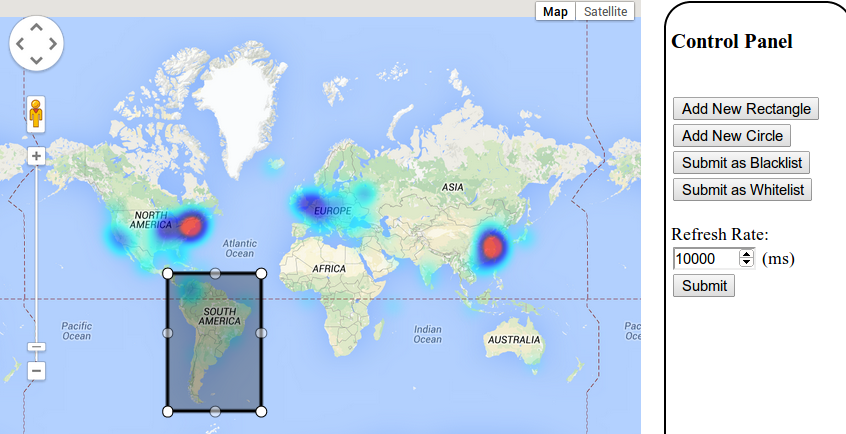
\includegraphics[width=\columnwidth]{control_panel.png}
\caption{\label{fig:map} A heatmap of static / historical data from a personal
web-server open to the Internet for the past few years.
The data was manually filtered to show only
suspicious activity, based on known legitimate usage of the server. The data may
however contain a number of false positives located in Pennsylvania and Boston,
the two primary locations the server was used.}
\end{figure}

\begin{figure}
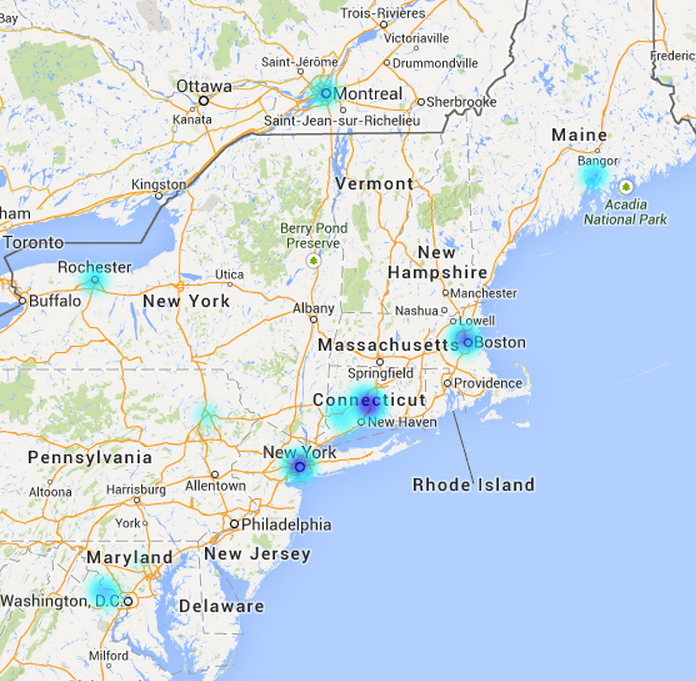
\includegraphics[width=\columnwidth]{NewEngland.png}
\caption{\label{fig:newengland} A zoomed-in version of Fig~\ref{fig:map} focusing
on the New England region. It is more apparent in this image the primary limitation
of our method. That is, the granularity of the geolocation data is limited to the
zip code in which an IP address is located.}
\end{figure}

Our prototype implementation has a javascript-driven web front-end which queries the
Google Maps API as seen in Fig~\ref{fig:map} with Fig~\ref{fig:newengland} showing just
the New England region. The figure contains a heatmap of, in
this case, static / historical data from a personal web-server. The more red a region
is, the more incidents there were that came from that region. This view of the data
gives the user a good feel for geographically similar incidents as well as number of
incidents occuring there.

\subsection{Interactivity}

Users can interact with the front-end by doing the following:

\begin{enumerate}
\item Create a rectangular or circular region on the map which can then be submitted
as a blacklisted or whitelisted region.
\item Changing the refresh rate of the page data.
\item Scroll and zoom the map just like any Google Map.
\end{enumerate}
%\subsection{Blacklisting and Whitelisting}
%\begin{enumerate}
%\item `Teaching' syntax for \verb+iptables+ using a separate HTML frame to contain
%a list of rules automatically generated based on what the user does to the map.
%\end{enumerate}

%\section{Applications}
%\subsection{Website Administration}
%\subsection{Big Data}

\section{Future Work}
\label{sec:future}

In this section we give lists of possible ways to improve on our proof-of-concept prototype,
in particular what analysis can be easily automated without the need for complicated
algorithms, and in what ways we can better give the user feedback to how the rules he or
she came up with are playing out on the network.

In Section~\ref{sec:collection}, we described the most basic kind of blacklisting rule
possible using \emph{ip2location\_ruby}; regional IP address based blacklisting. The
database available using this ruby gem however is not limited to (IP,geolocation) tuples.
The following rules could also be implemented:

\begin{enumerate}
\item Regional country / nation based filtering. Although the content provider can easily select
a rectangular region around a particular country, it may be more useful in certain
situations to be able to select a region by country. The ip2location ruby gem gives
a mapping from IP address to country / region which would allow for such filtering.
\item A content provider with a user-base concentrated in a specific locality / city
may wish to handle requests from the city in question on one powerful server, and
other requests on a separate slower server. The `city' field available in the ip2location
database gives us this capability. The content provider can select a city from the map
or dropdown menu, and have the requests not from that city redirected to the secondary
server. From a security / defensive point-of-view this eliminates the useability impact of
the website on the majority of the user-base when an attack comes from outside the target city.
\item Along with the city-based filtering, \emph{ip2location\_ruby} has a zip code field,
giving the content provider more flexibility in how he or she provides the system with
filtering rules.
\item A `timezone' field is also available in \emph{ip2location\_ruby}, giving us easy
access to the time of day in the region from which a packet originated. A content provider
might come to expect certain traffic patterns based on the time of day from a particular
region. Since network incidents tend to occur at random, without regard for normal
traffic patterns, the timezone field allows us to alert the content provider of anomalous-looking
traffic and let the content provider act accordingly.
\end{enumerate}

In Section~\ref{sec:collection} we also described how \emph{packetfu} is used to parse
packets taken from the network stack. Given the other information \emph{packetfu} makes
readily available (all TCP and IP header fields of a given packet) a more versatile
implementation would compile useful statistics and trends seen over time. In the front-end
(the Google Maps visualization) we would then be able to present the statistics in a
meaningful way in relation to everything else being presented. The content provider could
for instance flag packets with high RTTs (round-trip times) and further investigate where
they are coming from and what the requests are for.

The ip2location database lookup API we used in our prototype uses a binary search tree
to store the IP address to geolocation information mapping. Since people rely on and
have grown to expect low latency over networks, the use of a binary search tree in ruby
is likely not a scalable solution when it comes to analyzing every single packet on a
network. One possibility is to pre-compute a hash table each time the content-provider
submits a new set of blacklist / whitelist rules from the web interface. This hash table
would map IP addresses to geolocation information in $O(1)$ time, making it a scalable
solution on high bandwidth networks. The hash table then need only be distributed to all the
gateway machines available, dividing up the workload while maintaining consistency of
the desired security policy.

Some of the future improvements to make on the visualization side are as follows.

\begin{enumerate}
\item Show live packet statistics and / or live graphs to help the user
correlate large traffic bursts with packet and data types.
\item Allow advanced users to edit \verb+iptable+ rules themselves. Would need to
do syntax verification and input cleansing to make sure only \verb+iptable+ rules
are performed.
\item Add a color-bar to indicate the exact rate at which requests are originating
from a given location.
\item A hover textbox feature for telling the user the exact rate at which requests
are originating from the location over which the mouse is hovering.
\end{enumerate}

\section{Conclusions}
Although geolocation based blacklisting is, in its' present form, a form of unverifiable
authentication (IP addresses can be spoofed), its' economic benefits cannot be denied.
As such, firewalls, blacklists, and IDSs are here to stay. It is therefore in our best
interest to come up with quick and easy techniques for improving the security of our
networks today rather than waiting for vulnerability patches and smarter algorithms.

\bibliography{sources}
%\input{sources.tex}

%\balancecolumns

\end{document}
